En las Fig. (\ref{fig:I02})---(\ref{fig:I08}) se muestran los regímenes permanentes de 
las oscilaciones forzadas por los voltajes \qtylist{7,30;7,13;7,05;6,95}{\volt}, para cada corriente de amortiguamiento \qtylist{0,2;0,4;0,6;0,8}{\ampere}. Los voltajes empleados
corresponden a la frecuencia de resonancia del péndulo de Pohl para las diferentes
corrientes. Los puntos naranjas en las figuras indican la amplitud de las oscilaciones con
respecto al tiempo.
\begin{figure}[H]
	\centering
	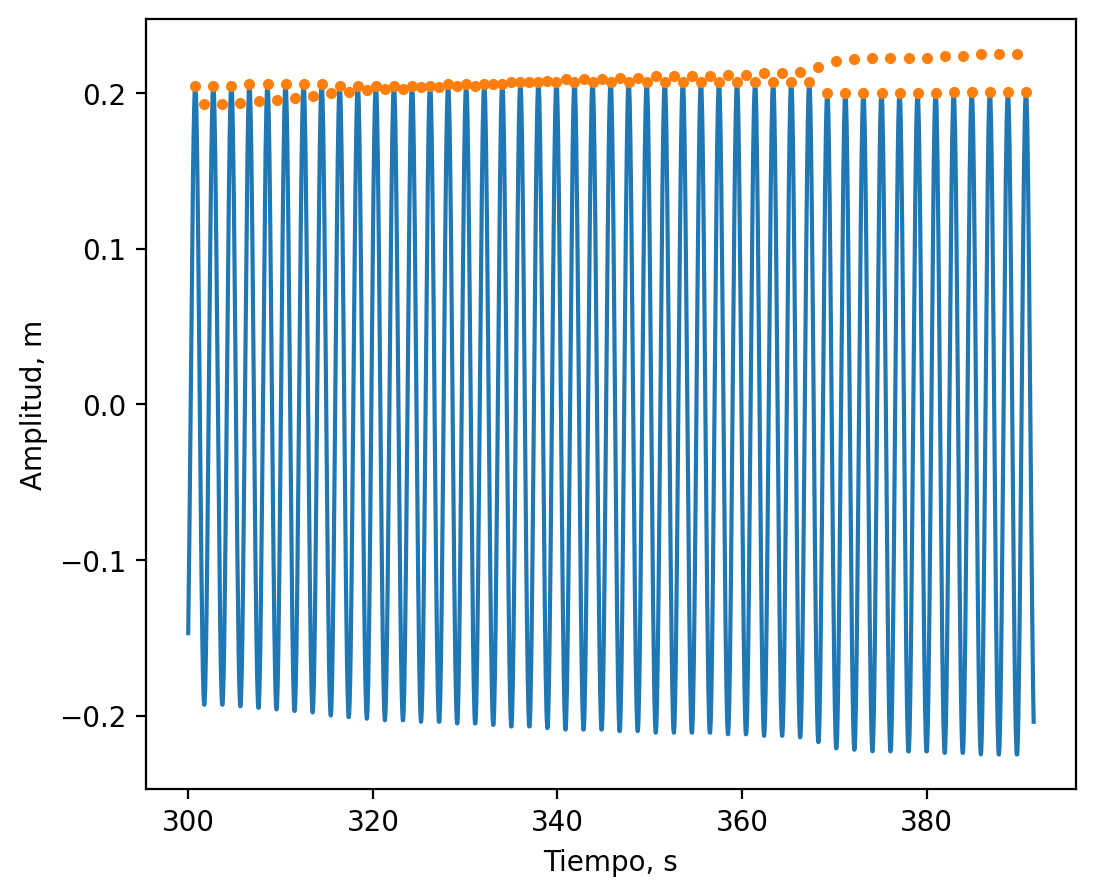
\includegraphics[width=\linewidth]{results/res/I02V73.png}
	\captionof{figure}{Régimen permanente de oscilaciones forzadas. $V$ = \qty{7,30}{\volt},
		$I$ = \qty{0,2}{\ampere}, $\bar{A}_M$ = \qty{0,2072}{\meter}.}
	\label{fig:I02}
\end{figure}

\begin{figure}[H]
	\centering
	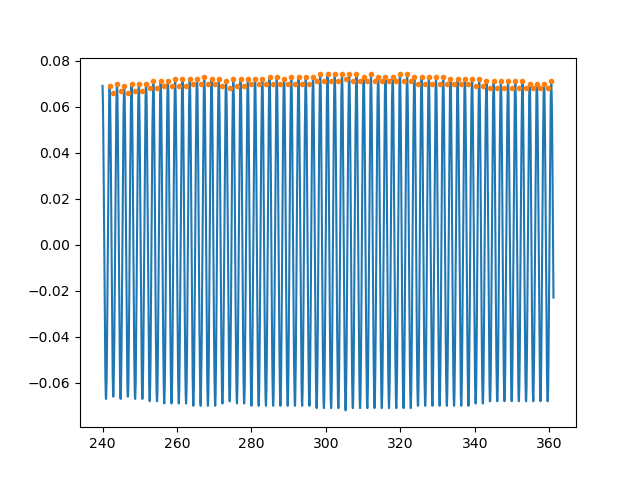
\includegraphics[width=\linewidth]{results/res/I04V713.png}
	\captionof{figure}{Régimen permanente de oscilaciones forzadas. $V$ = \qty{7,13}{\volt}, 
		$I$ = \qty{0,4}{\ampere}, $\bar{A}_M$ = \qty{0,07074}{\meter}.}
	\label{fig:I04}
\end{figure}

\begin{figure}[H]
	\centering
	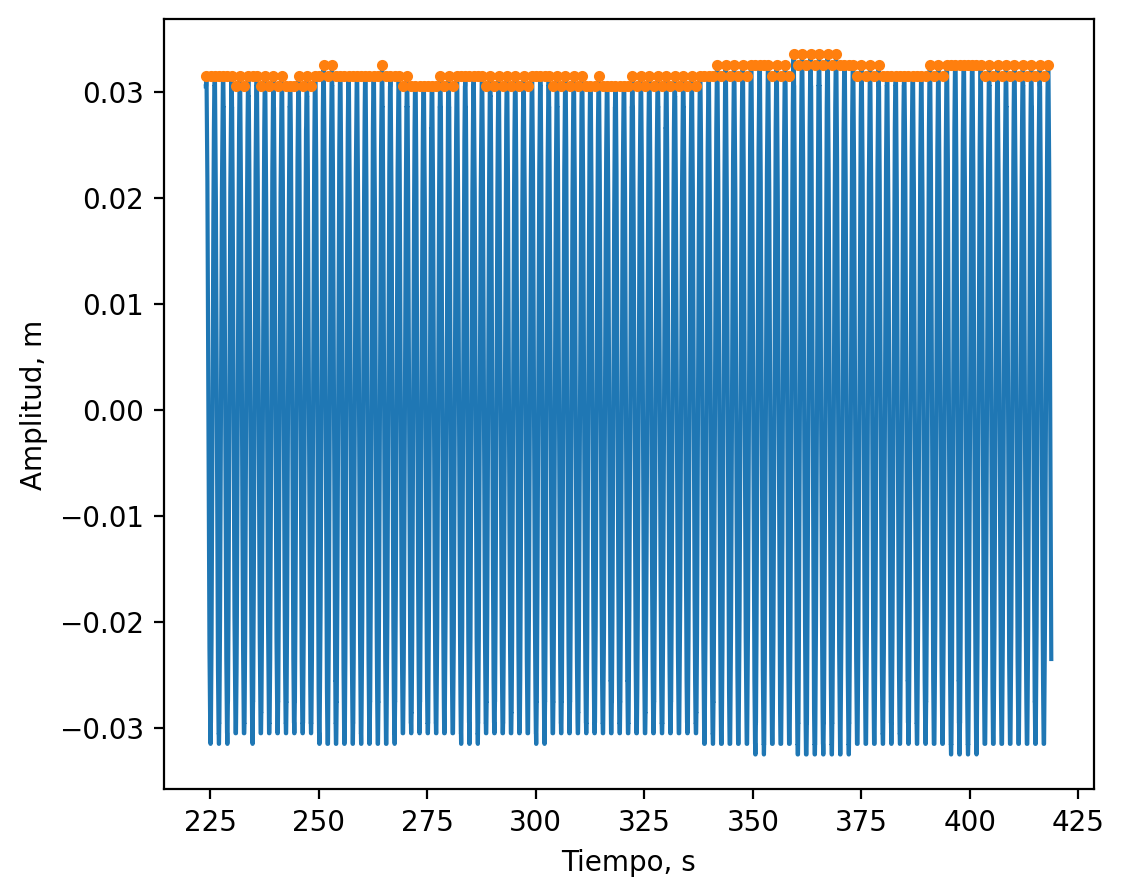
\includegraphics[width=\linewidth]{results/res/I06V705.png}
	\captionof{figure}{Régimen permanente de oscilaciones forzadas. $V$ = \qty{7,05}{\volt},
		$I$ = \qty{0,6}{\ampere}, $\bar{A}_M$ = \qty{0,03154}{\meter}.}
	\label{fig:I06}
\end{figure}

\begin{figure}[H]
	\centering
	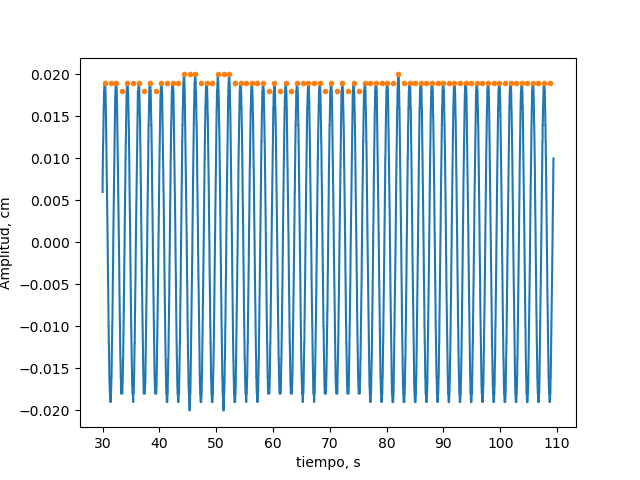
\includegraphics[width=\linewidth]{results/res/I08V695.png}
	\captionof{figure}{Régimen permanente de oscilaciones forzadas. $V$ = \qty{6,95}{\volt},
		$I$ =  \qty{0,8}{\ampere}, $\bar{A}_M$ = \qty{0,01896}{\meter}.}
	\label{fig:I08}
\end{figure}